\documentclass[11pt,a4paper]{article}
\usepackage[utf8]{inputenc}
\usepackage[T1]{fontenc}
\usepackage{lmodern}
\usepackage{amsmath}
\usepackage{amsfonts}
\usepackage{amssymb}
\usepackage{graphicx}
\usepackage{float}
\usepackage{listings}
\usepackage{xcolor}
\usepackage{geometry}
\usepackage{hyperref}
\usepackage[english]{babel}
\usepackage{caption}

\geometry{margin=2.5cm}

\definecolor{codeblue}{rgb}{0.25,0.5,0.75}
\definecolor{codegray}{rgb}{0.5,0.5,0.5}
\definecolor{codepurple}{rgb}{0.58,0,0.82}
\definecolor{backcolour}{rgb}{0.95,0.95,0.92}

\lstdefinestyle{mystyle}{
    backgroundcolor=\color{backcolour},
    commentstyle=\color{codegray},
    keywordstyle=\color{codeblue},
    numberstyle=\tiny\color{codegray},
    stringstyle=\color{codepurple},
    basicstyle=\ttfamily\footnotesize,
    breakatwhitespace=false,
    breaklines=true,
    captionpos=b,
    keepspaces=true,
    numbers=left,
    numbersep=5pt,
    showspaces=false,
    showstringspaces=false,
    showtabs=false,
    tabsize=2
}
\lstset{style=mystyle}

\title{Should I attack in Risk? (The Board Game)}
\author{}
\date{}

\begin{document}
    \maketitle


    \section*{tl;dr}
    I played around a bit trying to calculate what can happen when a country attacks another one in risk.
    It turned out to be a fun problem to think about, so I did a bit of an overkill.
    Scroll down to see a few exemplary results!


    \section{Motivation and Rules}
    The Risk games in my circle of friends rarely came to an end.
    Furious negotiations, out-of-game brawls over broken contracts, but also endless dice rolls in epic 30 vs. 20 troops battles often kept the game going until deep into the night.
    Most of the time we would break off, document the score in order to play it out on another day and then never finish the game.
    The dice rolling in particular is a big problem, because we play with what we call "Die Michelsonsche Verzögerungstaktik".
    This is just like the official one, except that only one troop can be lost per dice roll:

    \textbf{The attacker rolls}
    \begin{itemize}
        \item 1 dice with 1 attacking troop (if there are $x$ troops on a land, he can attack with $x-1$)
        \item 2 dice with 2 attacking troops
        \item 3 dice with 3 or more attacking troops
    \end{itemize}

    \textbf{The defender rolls}
    \begin{itemize}
        \item 1 dice with 1 defending troop
        \item 2 dice with 2 or more defending troops
    \end{itemize}

    After attacker and defender rolled their dice, the highest of each is compared.
    If the defender's highest dice is equal to or higher than the attacker's highest dice, the attacker looses a troop.
    Otherwise, the defender looses one.

    When 30 attackers fight against 20 defenders, this really takes some time.
    So naturally the question arises: Can this be calculated?
    Of course!


    \section{Single Probabilities}
    The possible outcomes of a single dice roll can be calculated by simple counting of possible outcomes.
    In total there are 6 possible scenarios for (1v1, 1v2, 2v1, 2v2, 3v1 or 3v2 dice).
    With a couple of for-loops, this is quickly done, e.g. for the case 2 attackers vs 1 defender:

    \begin{figure}[H]
        \centering
        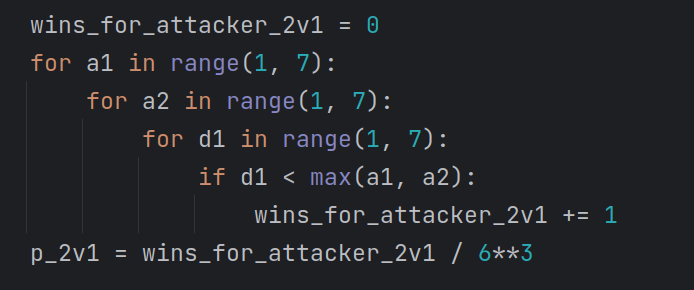
\includegraphics[width=0.6\textwidth]{../images/2v1.png}
    \end{figure}

    The probabilities for the attacker to win a single dice roll are:

    \begin{table}[H]
        \centering
        \begin{tabular}{|c|c|c|}
            \hline
            \textbf{attackers \textbackslash\; defenders} & \textbf{2 or more} & \textbf{1} \\
            \hline
            \textbf{3 or more}                            & 47\%               & 66\%       \\
            \hline
            \textbf{2}                                    & 39\%               & 58\%       \\
            \hline
            \textbf{1}                                    & 25\%               & 42\%       \\
            \hline
        \end{tabular}
    \end{table}

    Not too impressive for the attacker if you ask me!


    \section{Complete Attacks}
    Now that we have the single probabilities, the next step is to think about an entire attack: What is the probability to win with $a$ attackers against $d$ defenders?

    \subsection{Top Down}
    The first idea that comes to mind is recursion:

    To lead from $a$ vs $d$ to either victory (? vs 0) or defeat (0 vs ?), all possible paths have to be calculated, weighed with their individual probability and summed up.
    But from a local perspective, this simplifies as there are really only two possibilities: You either win a single roll or you loose one:

    \begin{figure}[H]
        \centering
        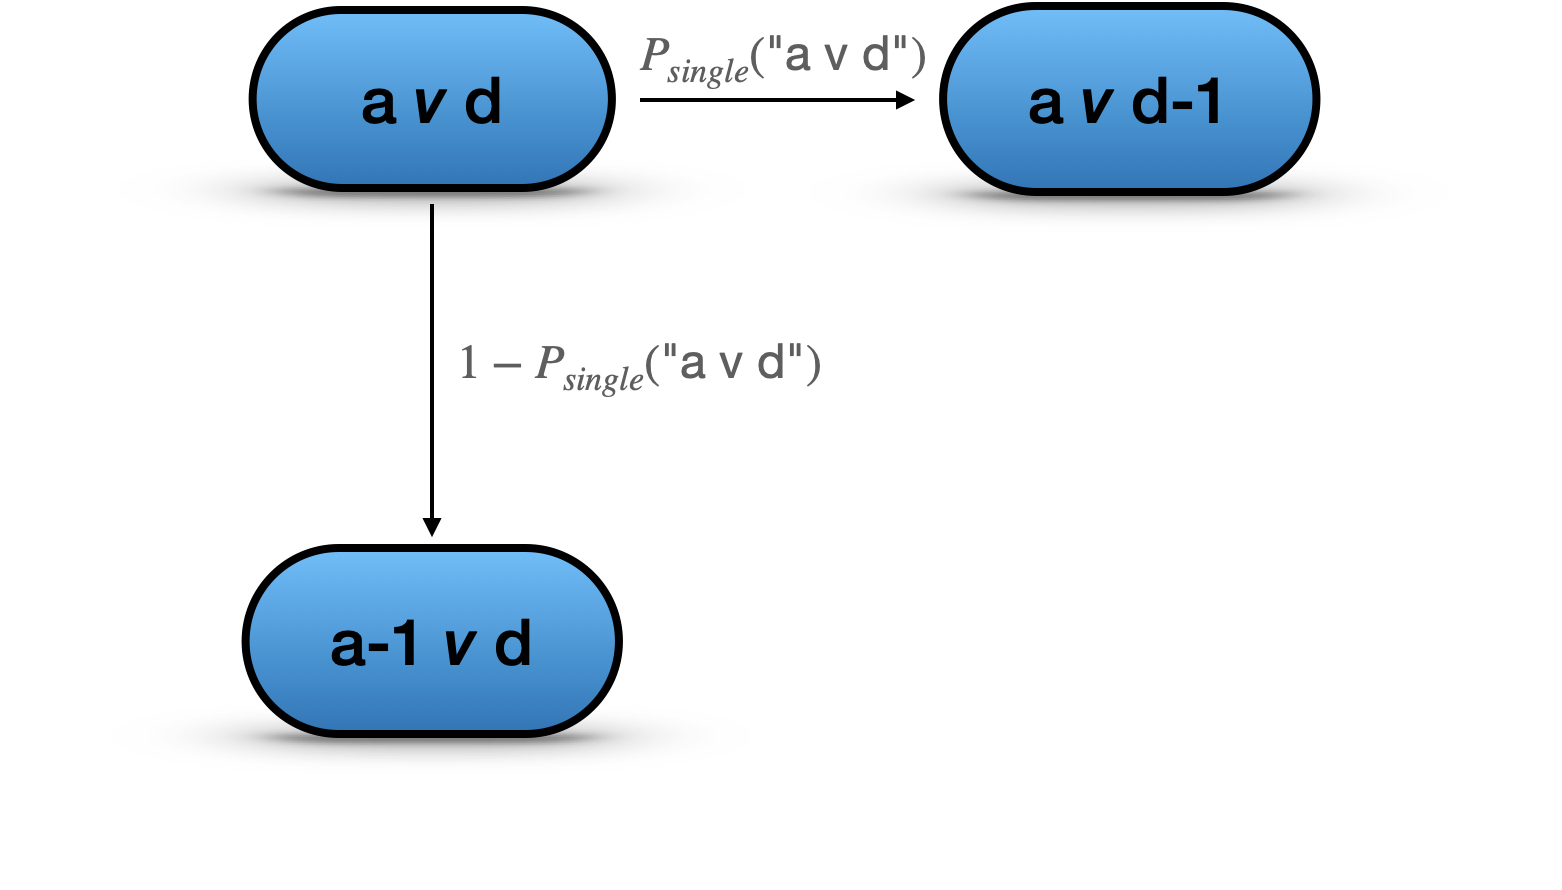
\includegraphics[width=0.6\textwidth]{../images/Basic Recursion.png}
    \end{figure}

    So the relation is obvious:
    \[ \begin{aligned}
           P_{total}(\text{``$a$ vs $d$''}) = &\; P_{single}(\text{``$a$ vs $d$''}) \cdot P_{total}(\text{``$a$ vs $d-1$''}) \\
           &+ (1 - P_{single}(\text{``$a$ vs $d$''})) \cdot P_{total}(\text{``$a-1$ vs $d$''})
    \end{aligned} \]

    The base cases are where no attacker or defender is left:
    \[ \begin{aligned}
           P_{total}(\text{``$a$ vs 0''}) &= 1 \; \text{ and}\\ P_{total}(\text{``0 vs $d$''}) &= 0 \\ \forall{a, d \geq 1}
    \end{aligned} \]

    In code, this is even easier to read:

    \begin{figure}[H]
        \centering
        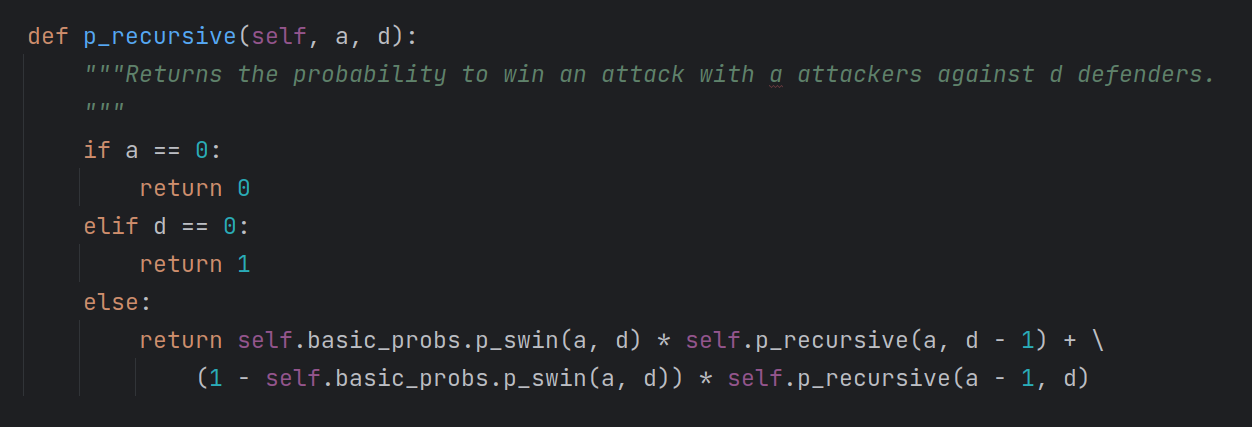
\includegraphics[width=0.6\textwidth]{../images/Recursive.png}
    \end{figure}

    For small attacks, this works just fine.
    For example, $P_{total}(\text{``10 vs 10''}) = 36.9\%$ (which is surprisingly low).
    But when the numbers increase, e.g. with 15 vs 15 my laptop already gives up.
    But why?

    It turns out, by design this 2d recursion scales pretty catastrophically.
    The first node gets called only once, but subsequent ones get called increasingly often:

    \begin{figure}[H]
        \centering
        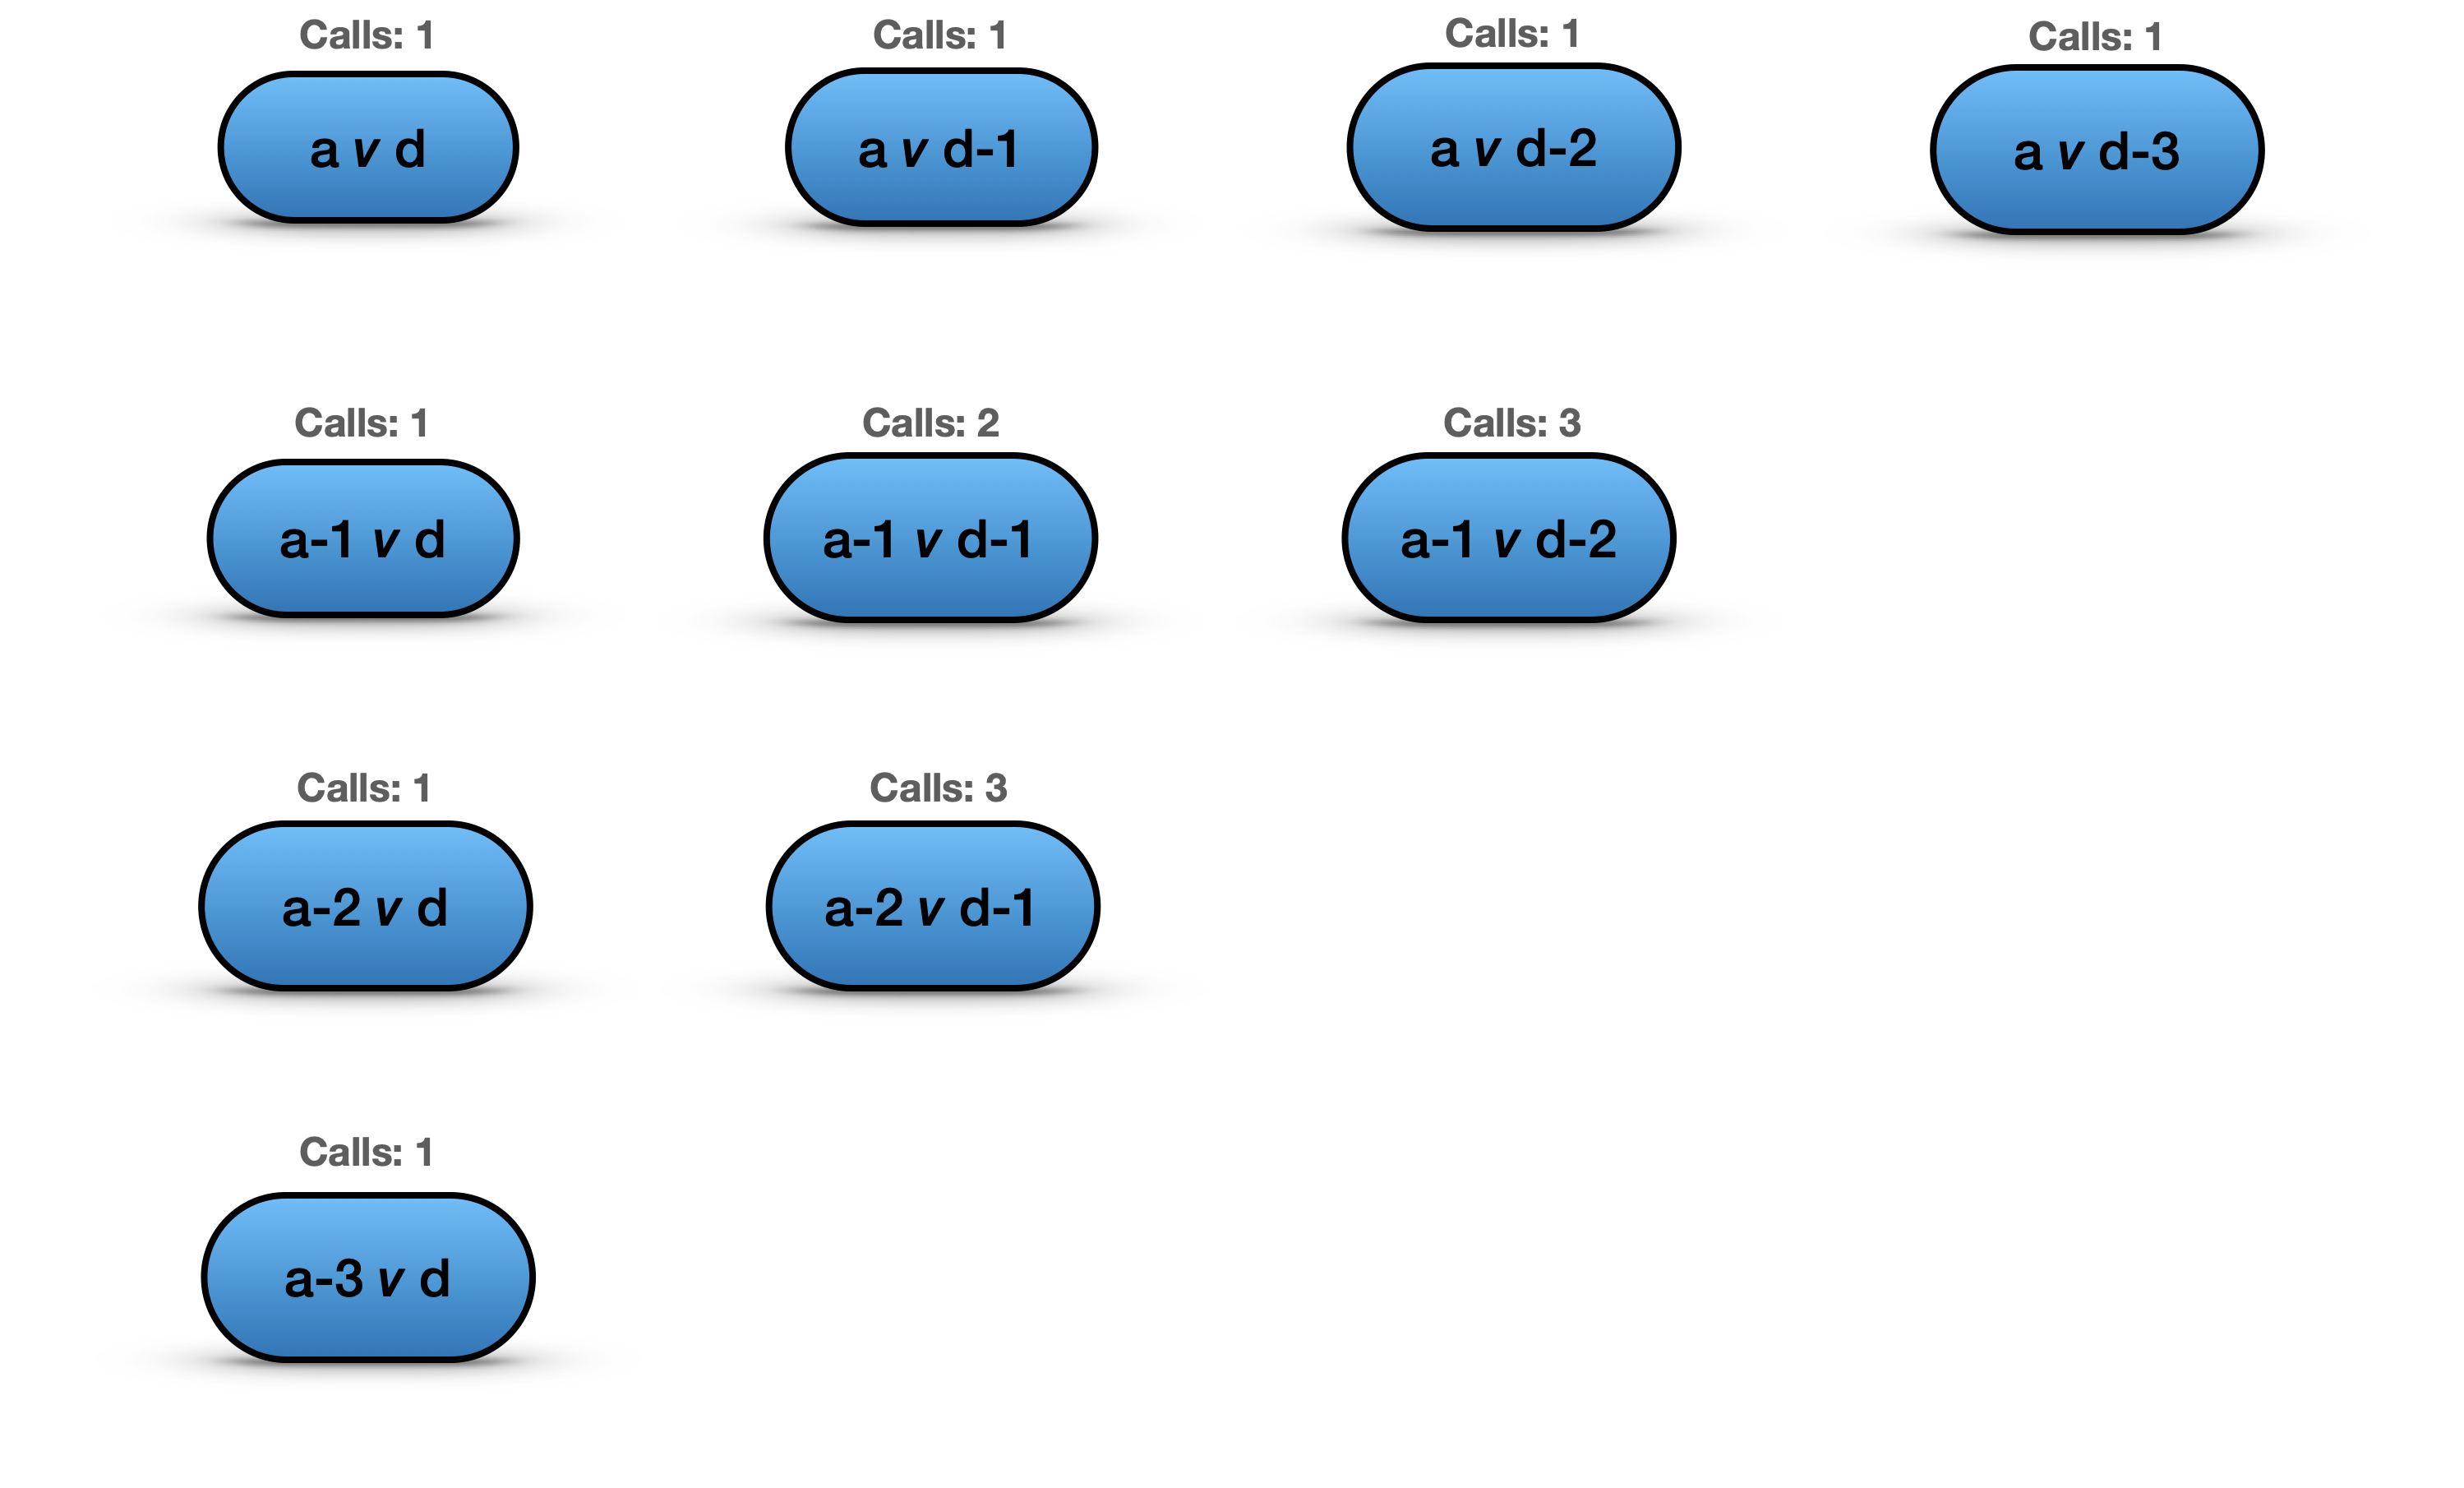
\includegraphics[width=0.8\textwidth]{../images/Pascal.png}
    \end{figure}

    Notice that each number of calls is of course just the sum of the number of calls for the node above and the one on the left of the current one.
    The ones on the outside can only get called once each, as they only have one left or upper neighbor.

    \begin{figure}[H]
        \centering
        
\includegraphics[width=0.7\textwidth]{../images/pascale meme2.jpg}
        \caption*{Pascal's triangle appeared out of nowhere!}
    \end{figure}

    So how many possible paths are there to get from the starting field to another one, assuming that they have a difference of $a$ attackers and $d$ defenders?
    \[ M(a, d) = \frac{(a + d)!}{a! d!} \]

    This can be shown with induction, using the previous equation as Induction Hypothesis (IH):
    The start with $(a, d) = (0, 1)$ or $(1, 0)$ is trivial.
    Now going from $(a, d)$ $(a+1, d)$:
    \[ \begin{aligned}
           M(a+1, d) & = M(a, d) + M(a+1, d-1) \\ & \overset{\mathrm{IH}}{=} \frac{(a + d)!}{a! d!} + \frac{(a+1 + d-1)!}{(a+1)! (d-1)!} \\ & = \ldots \\ & = \frac{(a+1 + d)!}{(a+1)! d!}
    \end{aligned} \]

    This is symmetric w.r.t exchanging $a$ and $d$, since the critical step in line 2 applies equally (any field can be reached from the fields left and above of it).
    When fighting with 30 against 20, the field (1, 1) alone is called $\frac{(29 + 19)!}{29! \cdot 19!} \approx 10^{13}$ times.
    No wonder my laptop gave up!

    Although I didn't realize it at the time I initially did this calculation (it was pretty much my first program), the easiest solution would be to use a cache, e.g. the \texttt{functiontools.lru\_cache} decorator.
    The value of each node is calculated only once and looked up from the cache when needed again.
    This means that all child calls that would be triggered on subsequent calls fall away too, and therefore it should solve the whole issue.

    But instead I came up with this idea, that works as well:
    One can change the conceptual view of going top down towards starting at the possible outcomes and working one's way up towards the initial starting point:

    \subsection{Bottom Up}
    The basic idea is to work from the bottom up.
    Given the probabilities in the fields under and on the right of any field, the probability to win starting from there can be calculated with exactly the same relation as before.
    The difference is just to start at the bottom.
    There the probabilities are already known, which sets up the boundary conditions:

    \begin{itemize}
        \item Wherever $a=0$, no attackers are left and $P=0$ (visualized in red, for unsuccessful attack)
        \item Wherever $d=0$, no defenders are left and $P=1$ (visualized in green)
    \end{itemize}

    \begin{figure}[H]
        \centering
        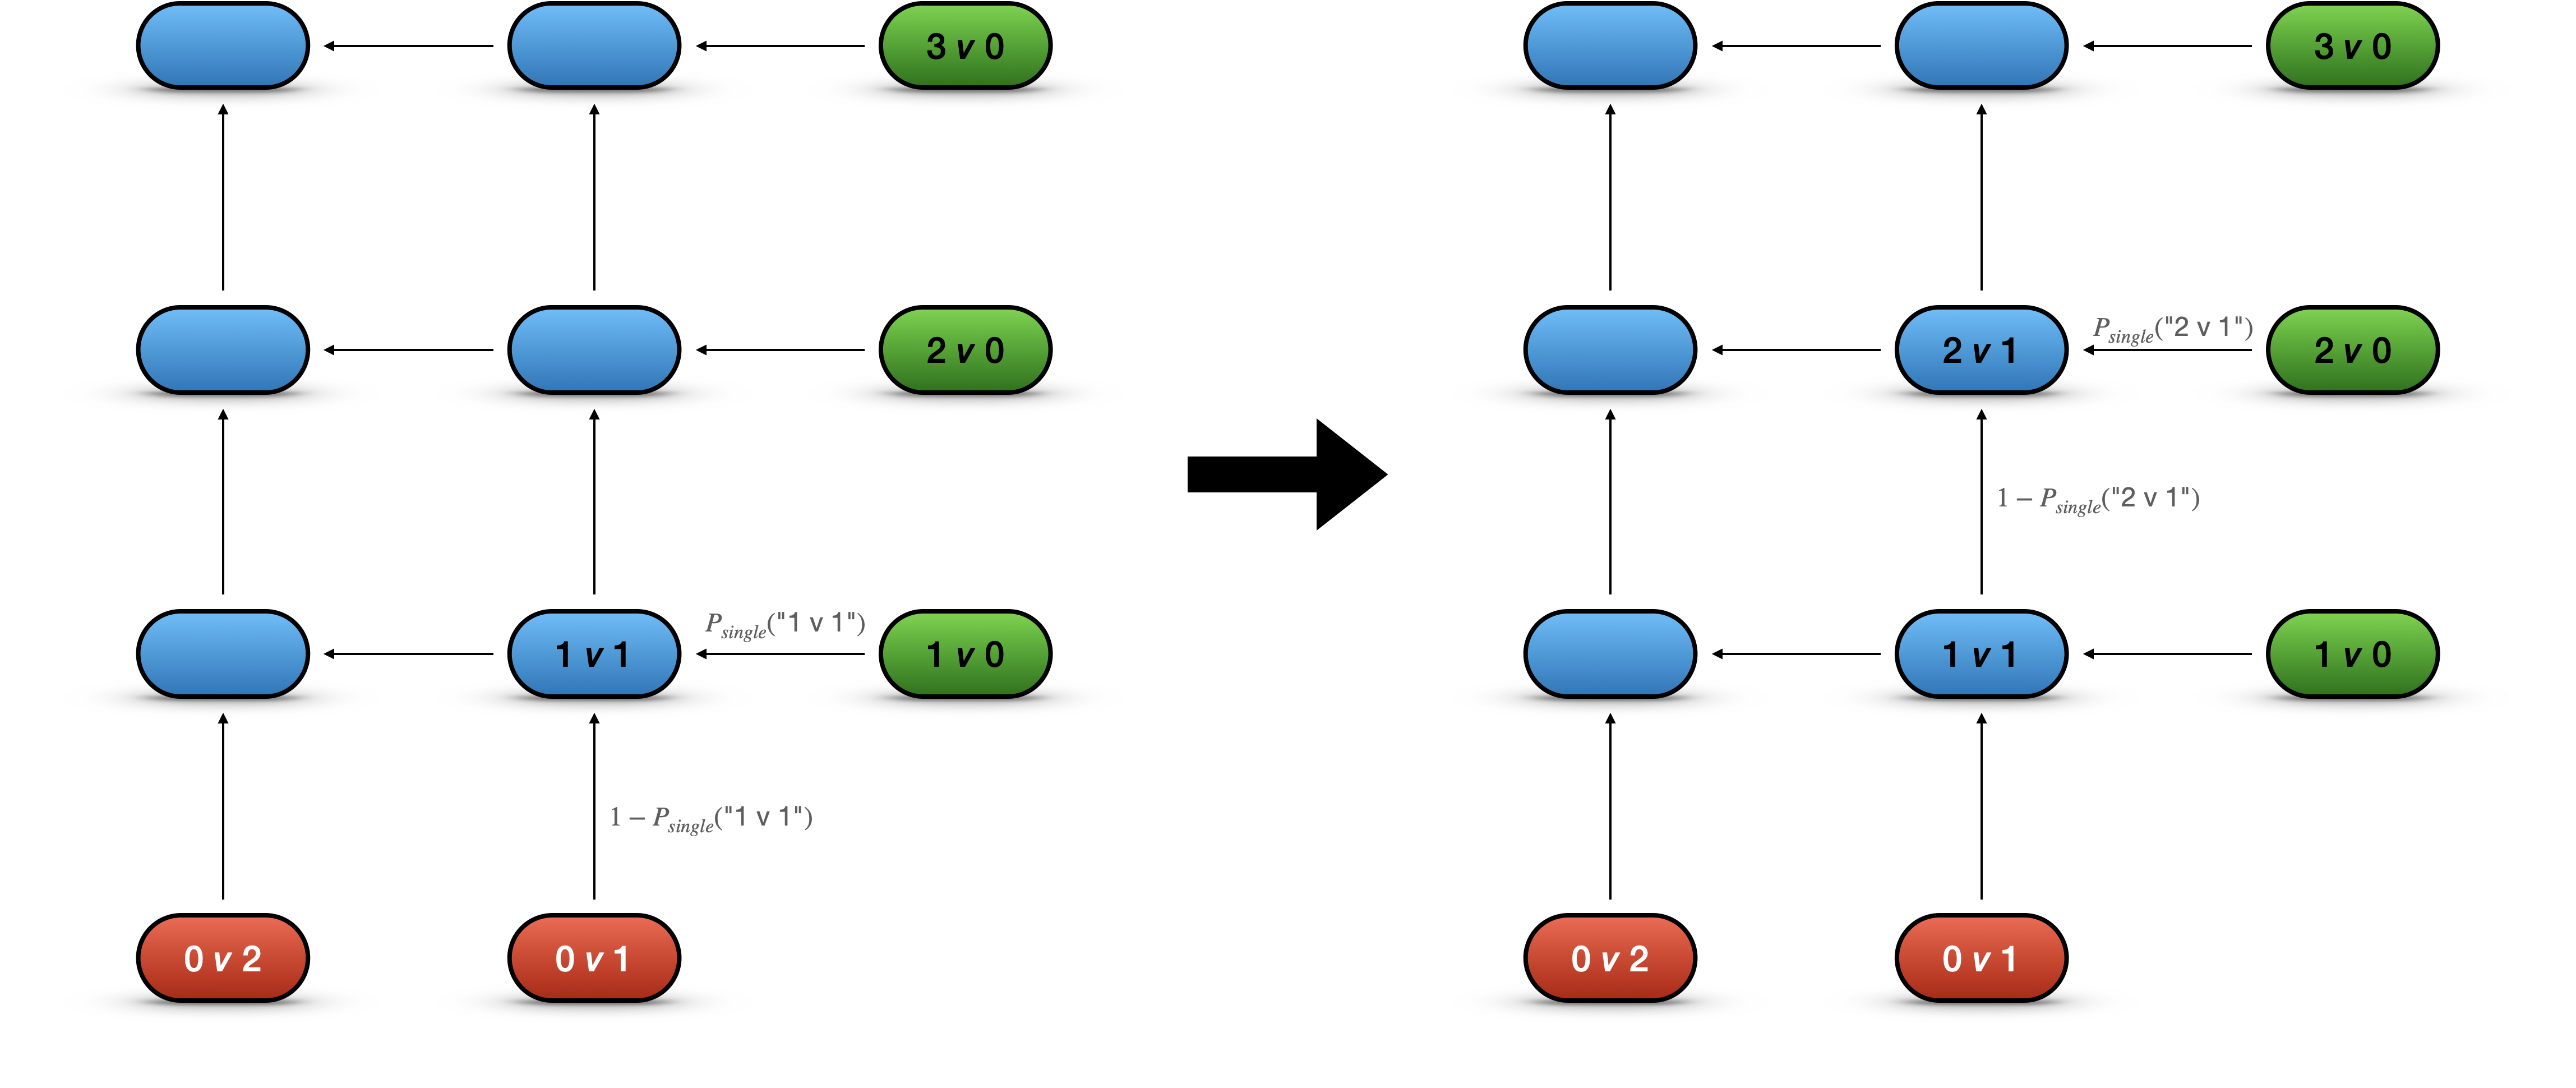
\includegraphics[width=1.0\textwidth]{../images/bottom up transition.png}
    \end{figure}

    And so on: Now it can just be iterated from the bottom right going up the columns right to left or the rows bottom to top.
    All $a \cdot d$ fields must be filled up, but this time only once!
    Using this, values up to $\sim$1000 can easily be reached: $P_{total}(\text{``1000 vs 1000''}) = 0.05\%$ (for such large numbers the 47\% of a single 3v2 become very small)

    The idea of boundary conditions is also convenient because they now can easily be changed.
    For example to answer questions like \textit{"How probable is it to win with the attacker having exactly 3 remaining troops?"}, this would just mean changing all outcomes to red (or $P=0$), except for the one where $a=3$:

    \begin{figure}[H]
        \centering
        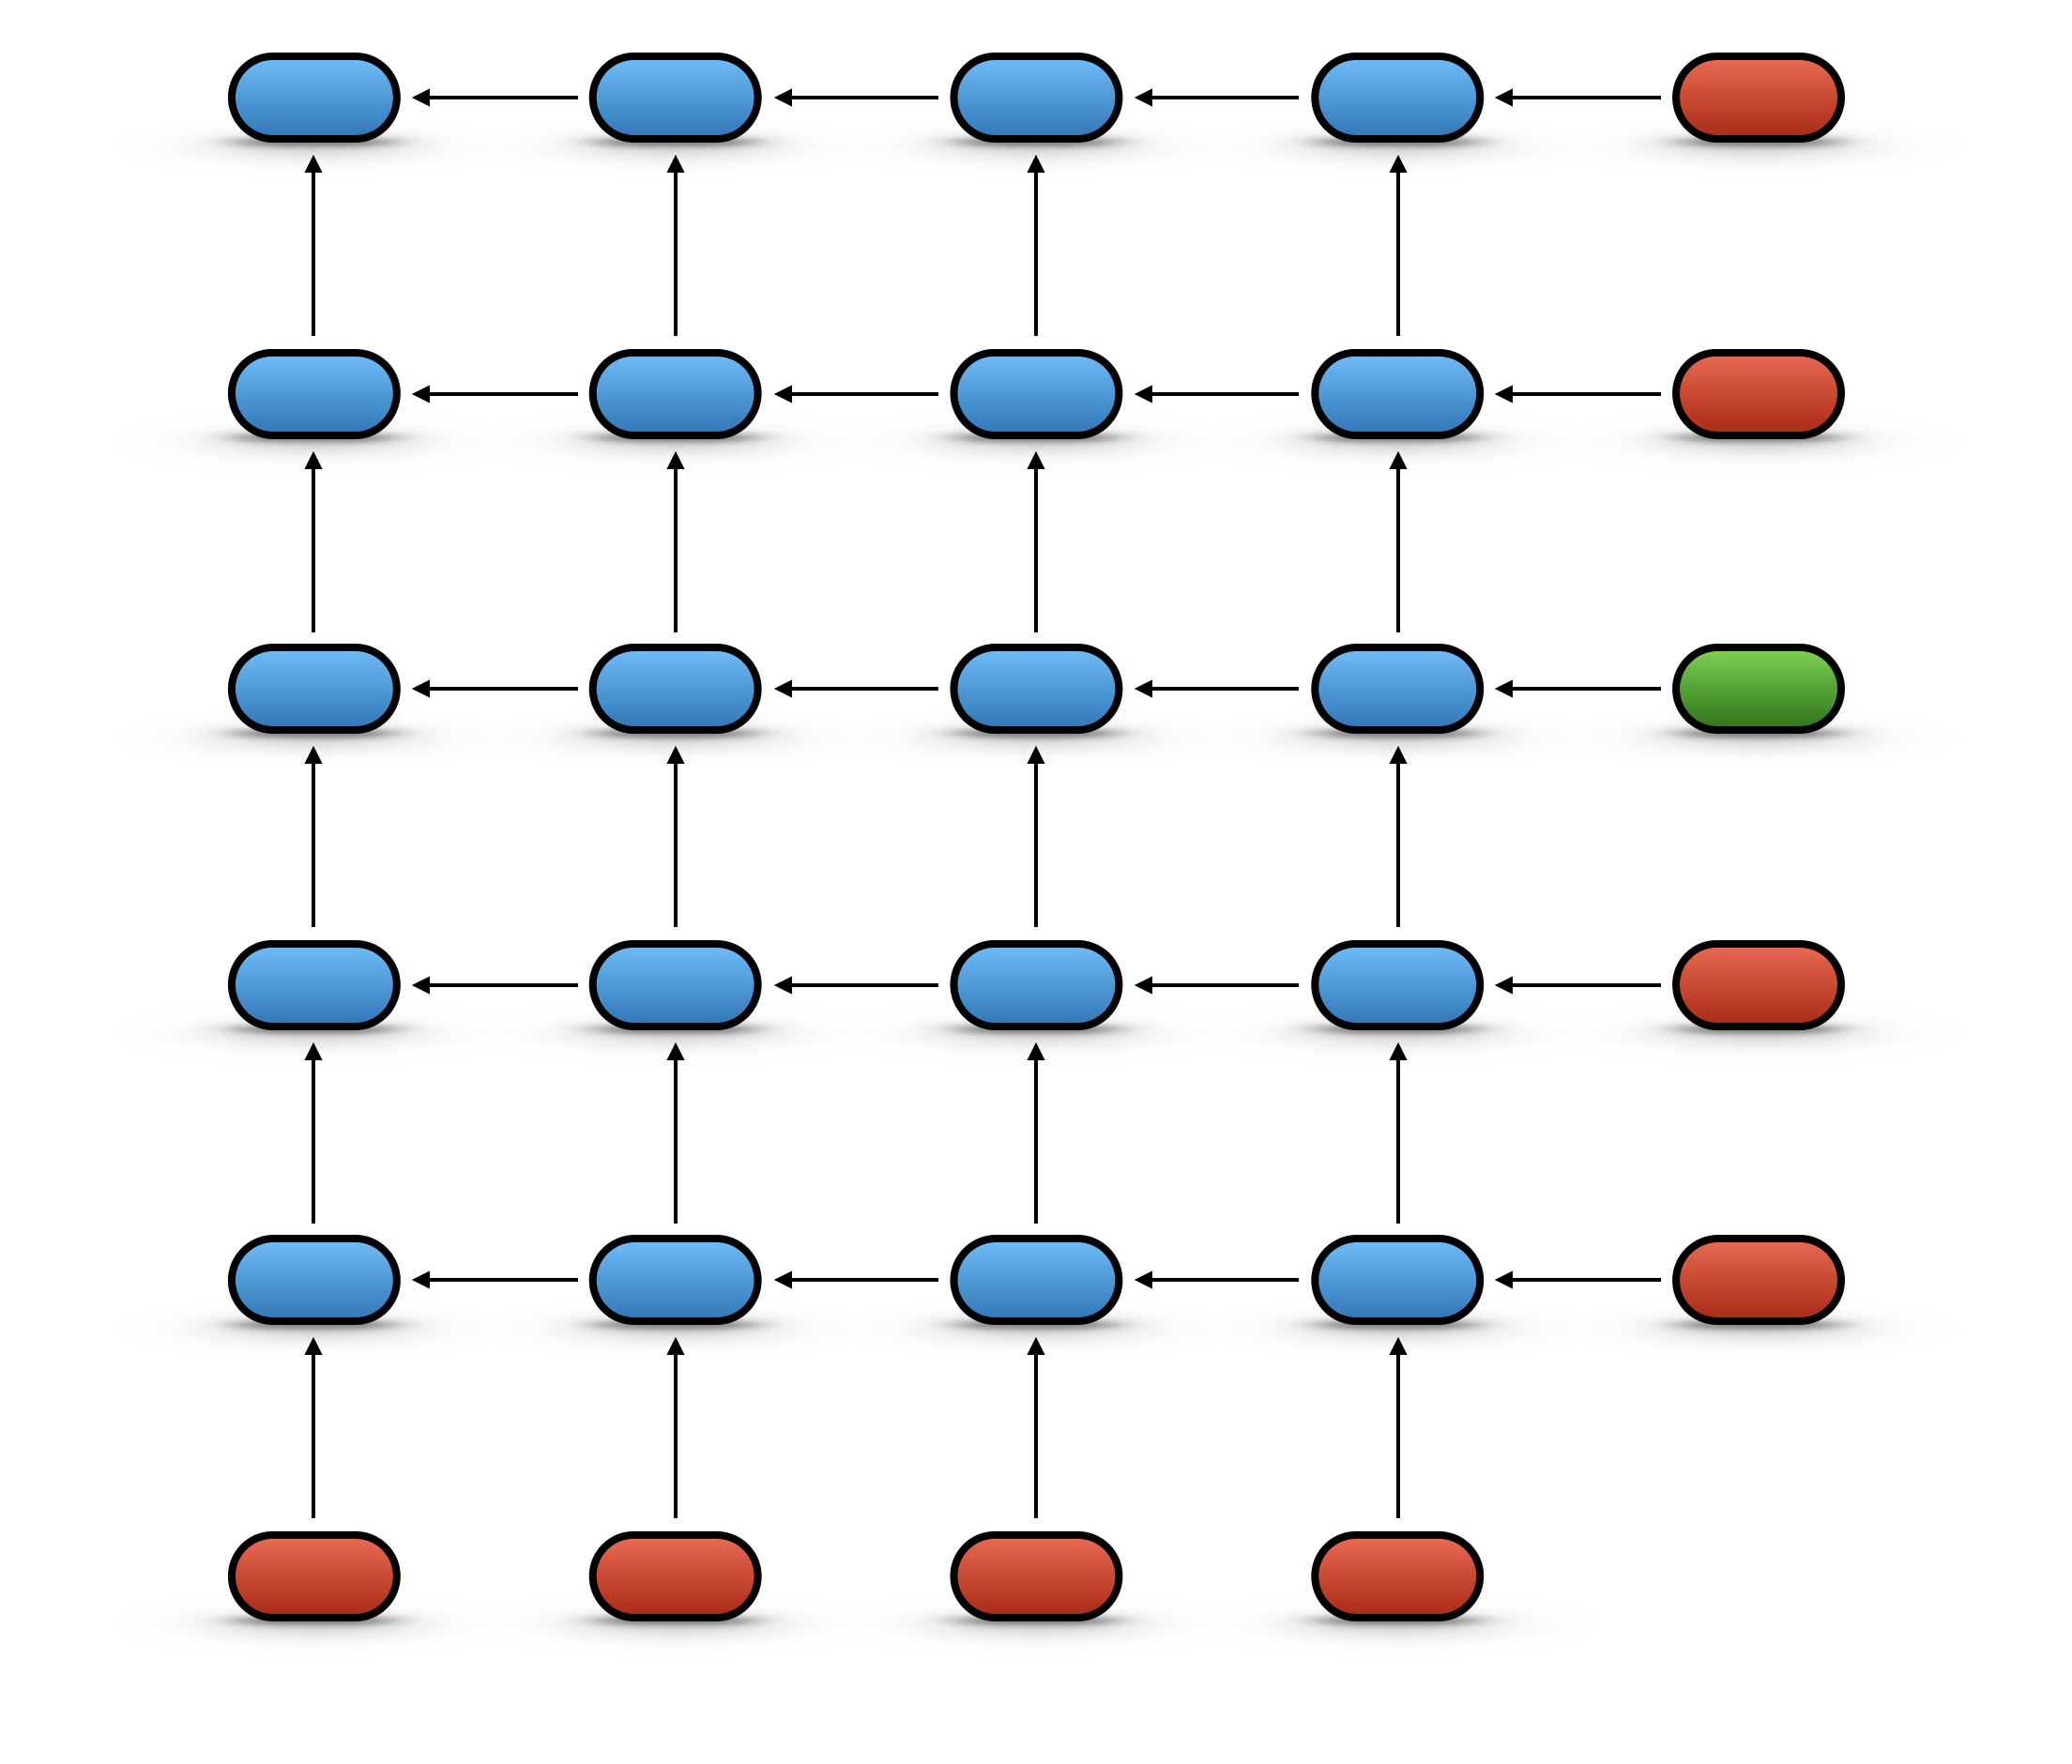
\includegraphics[width=0.6\textwidth]{../images/Boundary Conditions.png}
    \end{figure}


    \section{Results}
    Using this, here are some examples of attacking scenarios and the probabilities of each of their possible outcomes:

    \begin{figure}[H]
        \centering
        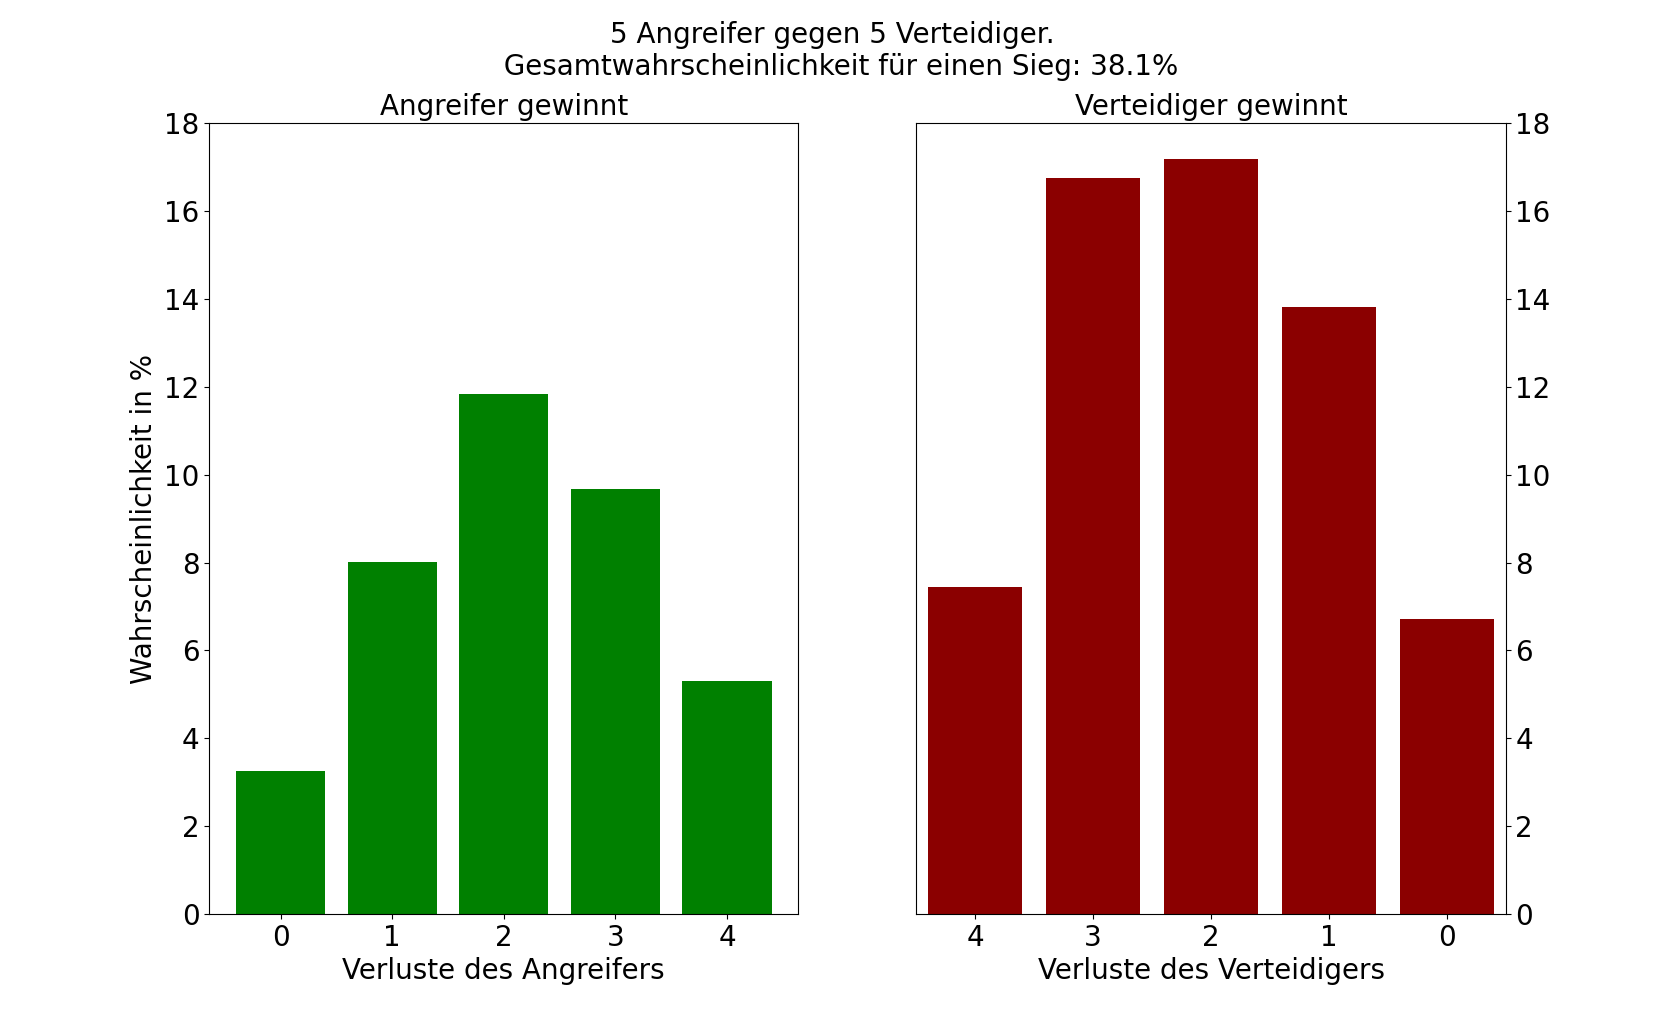
\includegraphics[width=0.9\textwidth]{../images/Risk5v5.png}
    \end{figure}

    \begin{figure}[H]
        \centering
        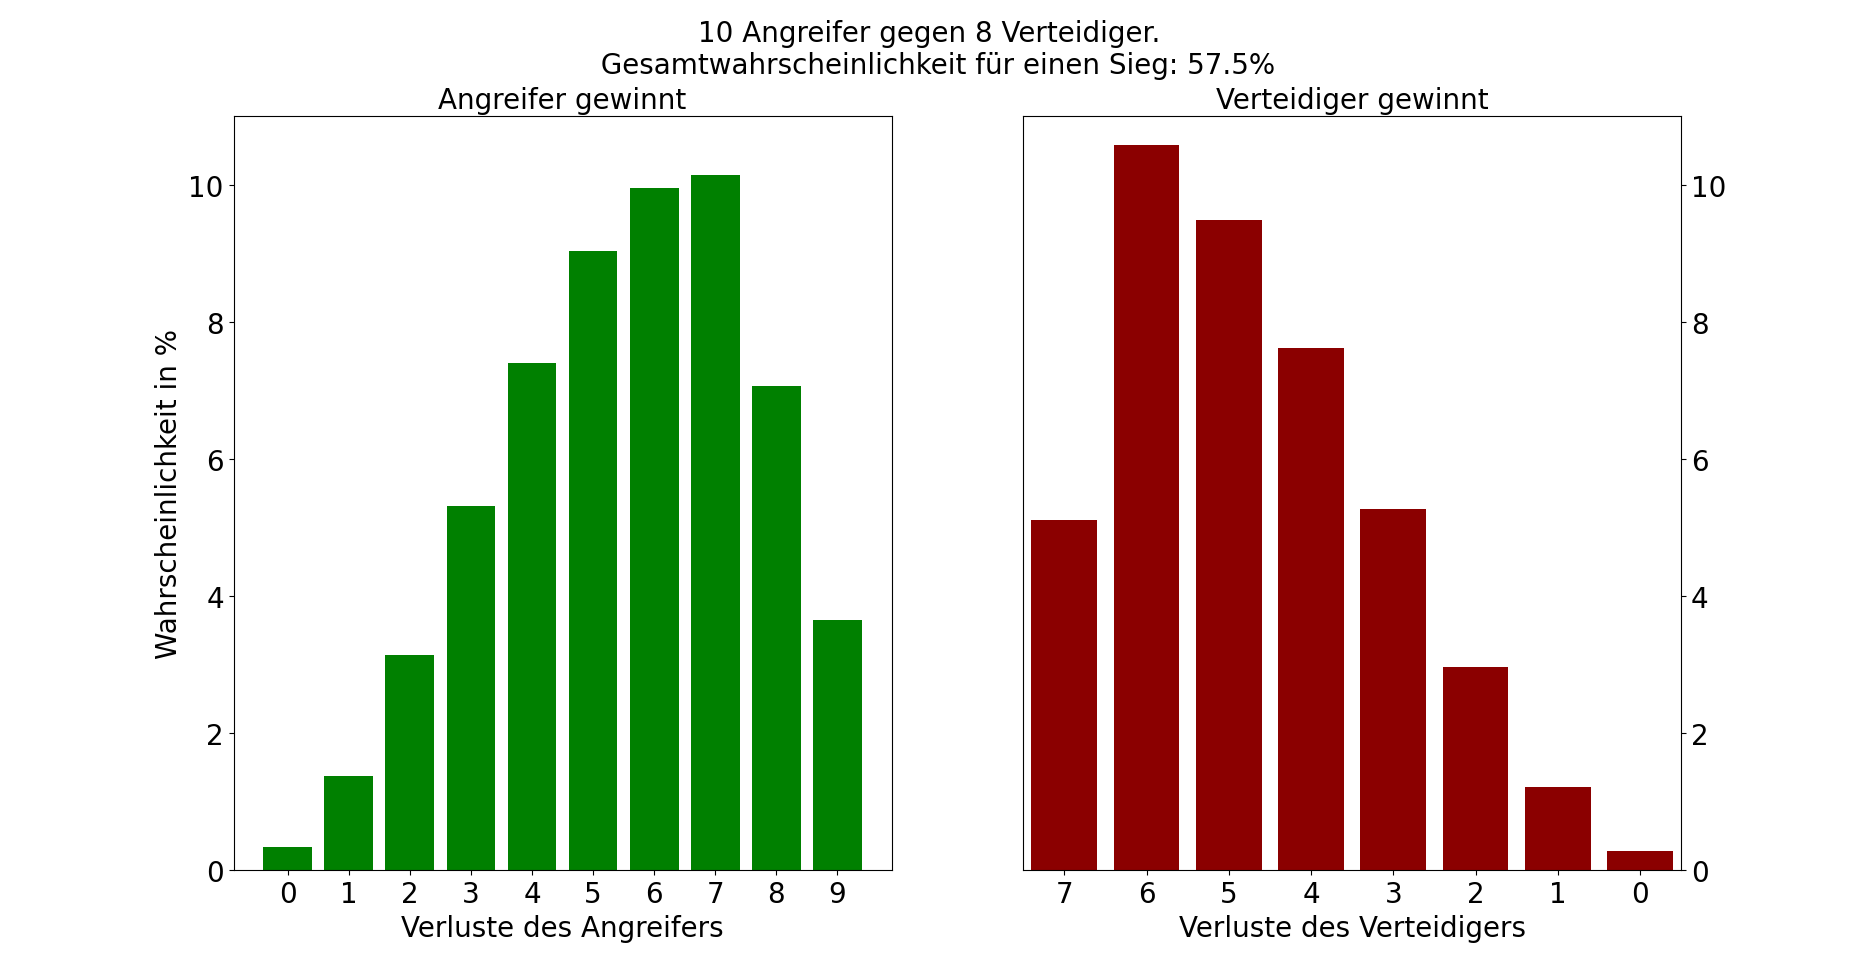
\includegraphics[width=0.9\textwidth]{../images/Risk10v8.png}
    \end{figure}

    \begin{figure}[H]
        \centering
        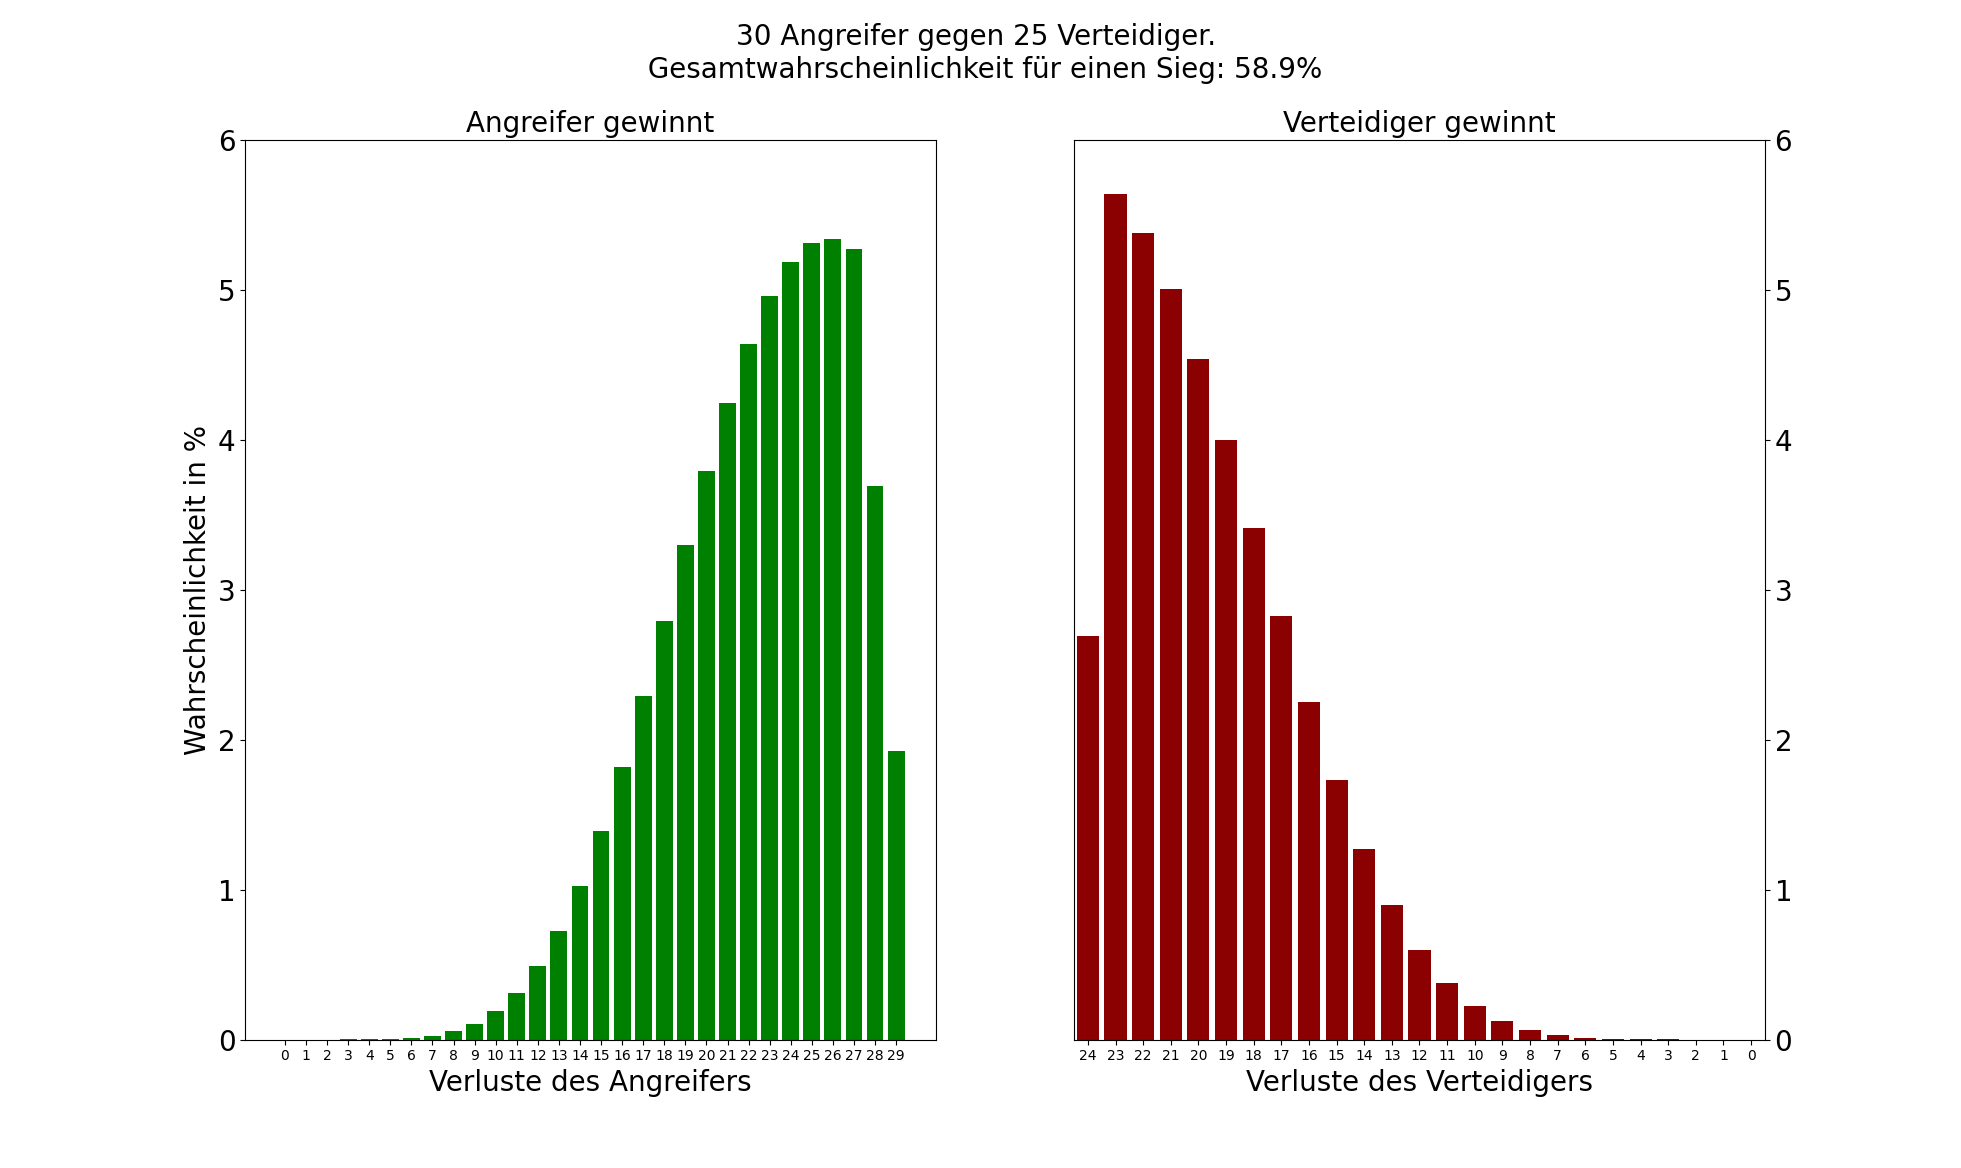
\includegraphics[width=0.9\textwidth]{../images/Risk30v25.png}
    \end{figure}

    What can be seen is almost a binomial distribution, but with dips where the attacker or defender runs into cases where the number of dice that can be used gets reduced.

    For smaller troupe sizes, what strikes me is that the curves are pretty flat.
    This reflects what we all know: Attacks are often just wildcards and everything can happen.


    \section{Conclusion}
    It is surprising how much time one can dump into something like this.
    But at least now we have the possibility to simulate the outcome of an attack within seconds instead of fifteen minutes.
    So for the first time, we started actually finishing games!
    Now that extinguishing a player happens within a second instead of in a 15 minutes crushing face-off, the threshold of doing so significantly reduced.
    Funnily enough a new threat came up in the later stages of the game: \textit{"If you attack me, I will not simulate"}, which means the whole table will have to wait for quite some time until they are done...


    \section{Outlook}
    Now that I've got a way to simulate 1000 vs 1000 one might say that's enough.
    This is of course not enough!

    To reach the really high numbers, an analytical approach would be necessary.
    It might work like this:

    \begin{figure}[H]
        \centering
        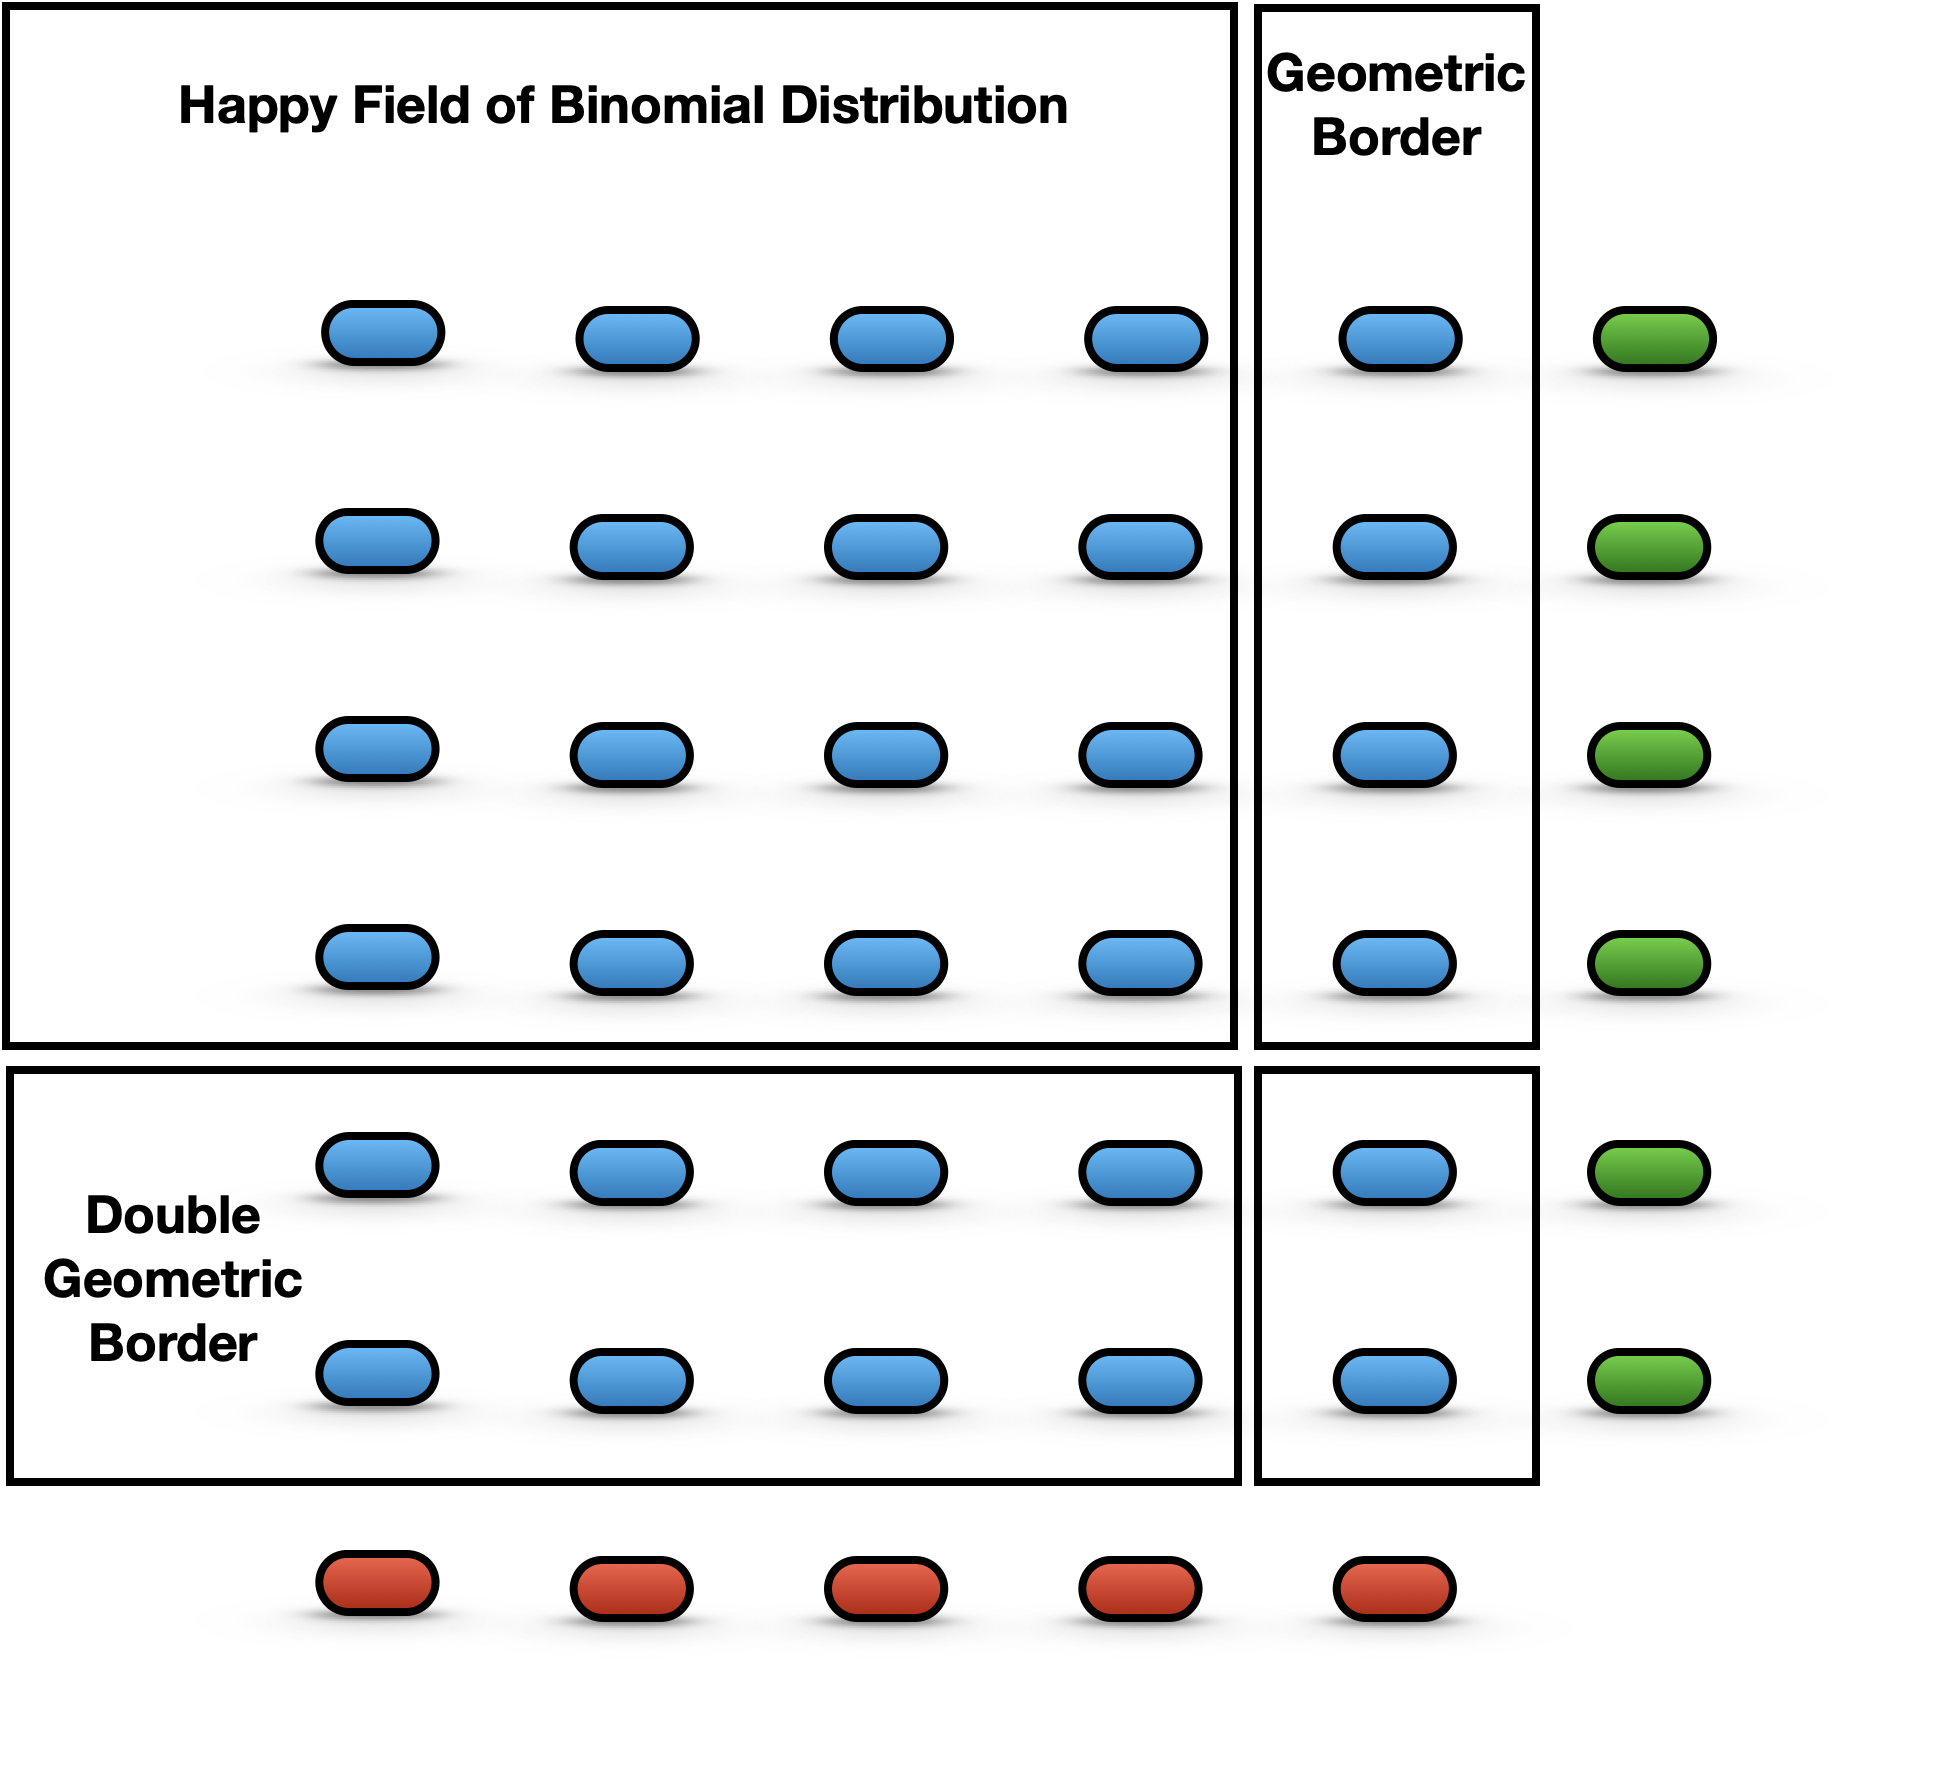
\includegraphics[width=0.8\textwidth]{../images/Analytic Interpolation.png}
    \end{figure}

    Within the Happy Field of Binomial Distribution, the probability of winning a single attack stays constant as the dice numbers don't change.
    So the probability to go from point A to point B can instantly be calculated using the binomial distribution.
    Then one would sum up all paths from the initial point to the border and weigh it the probability on the respective field on the border.
    For the right border ("Geometric Border"), this would come down to something like the geometric series, so it could be written down for each point.
    For the lower border, maybe some sort of "double" geometric series will come out... In total this seems pretty doable to me!


    \section{Addendum}
    About one and a half months after I posted this article as a TNG internal blogpost, Stephan Steinfurter, a friend and colleague of mine posted this fabulous answer, which is given here in original form:

    \vspace{\baselineskip}

    Thanks again for the nice problem.
    I was a little nerd-sniped ;).

    Indeed, one can obtain a solution linear in (a + d), exactly as you already outlined, Jonas.
    For the borders, there exist simple analytical solutions and the ``happy field of binomial distribution'' was in fact not happy at all for me.
    It was rather painful to get all the indices right.
    But in the end one indeed just needs the values on the borders and add them up with appropriate pre-factors (so, it is indeed just counting).
    But getting the binomial coefficients right is a bit nasty.

    I have a Jupyter notebook with all the nitty-gritty details.
    I may upload it to BitBucket, if anybody is interested.
    Here are the most important functions:

    \begin{lstlisting}[language=Python]
def Q_geometric_d_is_1(a, d):
    assert d == 1
    if a == 1:
        return p(1, 1)
    if a == 2:
        return p(2, 1) + (1 - p(2, 1)) * p(1, 1)
    return 1 - (1 - Q_dp(3, 1)) * (1 - p(3, 1))**(a-3)

def Q_geometric_a_is_1(a, d):
    assert a == 1
    if d == 1:
        return p(1, 1)
    return Q_dp(1, 2) * p(1, 2)**(d-2)

def Q_geometric_a_is_2(a, d):
    assert a == 2
    a_ = p(2, 2)
    b_ = (1 - p(2, 2)) * Q_dp(1, 2)
    c_ = p(1, 2)
    return Q_dp(2, 2) * a_**(d-2) + b_ * c_ * (c_**(d-2) - a_**(d-2))/(c_ - a_)
    \end{lstlisting}

    To obtain the last one from the previous, one needs to observe that Q(1, d) is a simple exponential and then use sth. like this formula.

    The rest is counting:

    \begin{lstlisting}[language=Python]
from math import comb
def Q_linear(a, d):
    return p(3, 3)**(d-1) * sum(comb(a + d - 4 - aa, d - 2) * (1 - p(3, 3))**(a - 2 - aa) * Q_geometric_d_is_1(aa+2, 1) for aa in range(a-2))
    \end{lstlisting}

    or as a formula:

    \[ \begin{aligned}
    Q_{ad} = &\; p_{33}^{d-1} * \sum_{a'=1}^{a-2} \binom{a + d - 4 - a'}{d - 2}(1 - p_{33})^{a-2-a'} * Q_{a'+2,1} \\
    &+ (1 - p_{33})^{a-2} \sum_{d'=1}^{d-1} \binom{a + d - 4 - d'}{d - 1 - d'} * p_{33}^{d-1-d'} * Q_{2,d'+1}
    \end{aligned} \]

    The binomial coefficients can be visualized in Pascal's triangle as the entries going up diagonally left/right from a particular point in the triangle. That particular point has N = (a - 3) + (d - 2) and k = d - 2 when written as ``N choose k''.

    Is it enough to compute Q(1000, 1000)?

    Well, in principle yes, sure.
    But in that particular version (\^{}), I get an ``OverflowError: int too large to convert to float'' for ``comb''.
    I guess, I will just have to switch to scipy's comb with ``exact=False'' or sth. like that.
    But who cares about the actual values...


\end{document}